
% The API of \sys\ is presented in Section~\ref{ssec:api}. 
Section~\ref{ssec:layout}  discusses \sys's data organization. 
We introduce mechanisms for supporting 
atomic scans  in Section~\ref{ssec:scans}, and describe \sys's
 normal (maintenance-free) operation flow  in Section~\ref{ssec:ops}.  
The data structure's maintenance is discussed in Section~\ref{ssec:rebalance}.
Finally, Section~\ref{ssec:flush-recovery} discusses flushing data to disk and failure recovery.


\subsection{Data organization}
\label{ssec:layout}

\begin{figure}[htb]
\centerline{
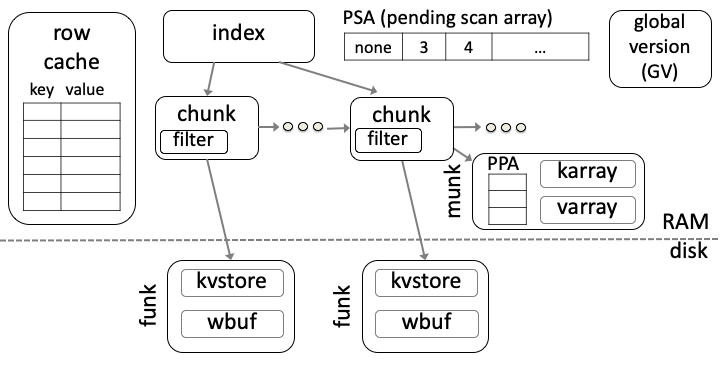
\includegraphics[width=\columnwidth]{PiWi.png}
}
\caption{\sys\ data layout.}
\label{fig:layout}
\end{figure}

\paragraph{Chunk-based layout.}

\sys's data layout is depicted in Figure~\ref{fig:layout}.
Similarly to BTrees {and other disk-friendly data structures}, 
\sys\ organizes data in fixed-size \emph{chunks}, each holding a contiguous key range.
This improves the efficiency of both disk access and memory access, in particular, for  range scans. 
At run-time, a list of all chunks is kept in RAM, where each chunk's data 
(consisting of keys in the corresponding range and values associated with them) 
is kept on disk (for persistence), and possibly in memory (for fast access). 

On disk, each chunk is associated with a  \emph{funk (file chunk)} as illustrated in 
Figure~\ref{fig:funk}. A funk
consists of two files:   
a compacted and sorted  key-value store \emph{kvstore} and a write buffer \emph{wbuf}. When a funk is created, the \code{kvstore} holds all the chunk's keys with corresponding values, and the \code{wbuf}  is empty.
New key-value pairs are subsequently appended to the unsorted \code{wbuf}. Note that if a key is over-written, it remains in the \code{kvstore} associated with the old value, and is included in the \code{wbuf} with the new one.
That is, the \code{wbuf} is more up-to-date.

\begin{figure}[htb]
\centerline{
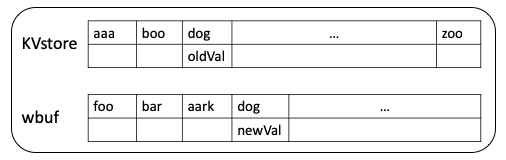
\includegraphics[width=\columnwidth]{funk.png}
}
\caption{A \sys\ funk consists of a sorted \code{kvstore} and an unsorted \code{wbuf} holding the most recent updates.}
\label{fig:funk}
\end{figure}

This structure allows us to benefit from sorted searches on the \code{kvstore}, and at the same time
allows for updating chunks without re-writing existing data, thus minimizing write amplification.
As a funk's \code{wbuf}  grows, however, searching becomes inefficient   and  
the funk is no longer compact, i.e., it may contain redundant (over-written) values.
Therefore, once the \code{wbuf}  exceeds a certain threshold, we reorganize the funk
via a process we call \emph{rebalance}, as explained below.



A subset of the chunks is also cached in memory to allow fast access, where each cached chunk is associated with a
\emph{memory chunk (munk)}  data structure. 
Munks are volatile and can be removed and recreated from funks at any time.
Thus, multiple \emph{generations} of munks may exist for a chunk throughout its life time.


At run-time, \sys\ holds in memory a linked list of chunk objects as well as 
%representing all funks in the data store. Chunks are also indexed in-memory for fast access by key using 
a \emph{chunk index}, which is a sorted map from keys to chunks (e.g., a sorted array, skip list, or search tree).
Note that since chunk objects do not hold actual keys and values, they are significantly smaller than munks and funks. 
\inred{A typical chunk object is smaller than 1KB, whereas the size of a funk or munk that holds 10K to 100K keys 
ranges between 1M to 100M depending on the data size.} 


A munk consists of two arrays -- \emph{karray} for keys and \emph{} for values. The  \code{karray}  holds a sorted linked list of the chunk's keys
with pointers to values in the \code{varray}. 
When a munk is created, its  \code{karray}  is sorted by key, so each cell's successor in the linked list is the ensuing cell in the array.
As new keys are added, they create bypasses in the linked list and  \code{karray}  is no longer sorted.
But if a sizeable portion of the  \code{karray}  is sorted, bypasses are short in expectation.
Key removals, in turn, leave obsolete values in the karrray, so it is no longer compacted.

As key-value pairs are added, overwritten, and removed munks and funks need to undergo reorganization. This includes  
(1) \emph{compaction} to deallocate removed and overwritten data, 
(2) \emph{sorting} keys to make searches more efficient,  
(3) \emph{splitting} overflowing chunks, and
(4) \emph{merging} under-utilized ones.
All reorganizations are performed by \sys's \emph{rebalance} operation.
If the chunk has a munk, then rebalance compacts and sorts the munk in-memory by creating a new 
(compacted and sorted) munk instead of the existing one. 
Funks of uncached chunks are also compacted by replacing them with new funks, albeit less frequently.
Splits  create new chunks as well as new  funks (and possibly munks) associated with them.

\paragraph{Expediting reads.}
As long as a chunk  is memory-resident, the munk data structure serves both the read-path and the write-path for keys in this chunk. 
In this case, the munk is quickly located using the index, and the  \code{karray}'s sorted prefix allows for efficient binary search.
Thus, \sys\ is particularly fast when almost the entire working set is memory resident. 
We take two measures to mitigate the performance penalty of accessing keys in munk-less   chunks, namely 
a row cache and Bloom filters, as we now explain.

First, we keep a \emph{row cache} holding popular key-value pairs. Note that unlike munks, which cache key ranges, the row
cache caches individual keys, and is thus more effective in dealing with point queries (gets as opposed to scans) with no
spatial locality (i.e., popular keys are not adjacent in the key space). \sys\ uses both data structures, and so 
popular key ranges are associated with munks (and can be scanned quickly), 
and  ``isolated'' popular keys are included in the row cache for efficient gets.

For working sets that are  larger than the available RAM size, these two caches might not suffice, and so a certain portion of reads will need to be served from disk. Here, the slowest step is the sequential search of the \code{wbuf}. 
If a key indeed resides in the 
\code{wbuf} (and is not cached in RAM), there is no way around that -- we need to locate it in the \code{wbuf} in order to find 
its associated value. However, we would like to reduce \code{wbuf} searches to a minimum. 
To this end, each chunk holds a \emph{Bloom filter} for the corresponding funk's \code{wbuf}; 
this is a statistical data structure that summarizes a set of keys so that 
when queried for a key that is included in it always returns true (no false negatives), 
and otherwise returns false with some high probability (low false positive probability). 
Thanks to these Bloom filters, we eliminate most of the redundant \code{wbuf}  searches.
In most workloads, \code{wbuf}  searches will be rare, as the \code{wbuf}  only includes keys written to the chunk 
since its last rebalance.

\paragraph{Synchronization structures.}

In addition to the chunk list and chunk index, \sys\ keeps a \emph{global version (GV)} for supporting atomic snapshot scans,
as described below; it tracks active scans in a \emph{pending scan array (PSA)} for garbage collection purposes (old 
versions not needed by any active scan can be reclaimed).

The chunk data structure is given in Algorithm~\ref{alg:chunk}. 
The first field is its status, which is explained  below. 
It next holds a pointer to the appropriate funk, and, if applicable, also munk, as well as a pointer to the next 
chunk in the chunk linked list.
It further keeps the generation number of its latest munk and a per-generation sequence number,
which, in case there is an active munk, is the index of the next free cell in the munk's  \code{karray}  and \code{varray}.
It further includes a Bloom filter as explained above.

\begin{algorithm}[htb]

\begin{algorithmic}
\State \code{status} \Comment  baby, child, active, asleep, or aged
\State ptr \code{funkPtr} \Comment funk disk address
\State ptr \code{munkPtr} \Comment munk memory pointer
\State ptr \code{next} \Comment next chunk in linked list
\State int \code{gen} \Comment munk generation
\State int \code{seq} \Comment sequence number in current generation 
\State \code{bloomFilter} \Comment summary of set of keys in the funk's \code{wbuf}
\State asymmetric lock \code{rebalanceLock} \Comment shared/exclusive lock 
\State lock \code{funkChangeLock} \Comment acquired with try\_lock 
\State \code{PPA[threads]} \Comment pending put array
\end{algorithmic}

\caption{Chunk data structure.}
\label{alg:chunk}
\end{algorithm}


The chunk additionally includes locks and data structures to synchronize concurrent access by multiple threads.
The replacement of a chunk (due to a split) or of a funk or munk associated with a given chunk 
must be executed atomically, and moreover, must be synchronized with concurrent puts. 
This is controlled by the chunk's \emph{rebalanceLock}, which is held for short time periods
during chunk, funk, and munk replacements.  It is a shared/exclusive lock (r/w lock), acquired in shared mode 
by put operations and in exclusive mode by rebalance. Gets and scans do not need to acquire the lock at all.

To minimize I/O, we allow at most one thread to rebalance a funk at a given time; this is controlled by 
the  funkChangeLock. This lock is used at a coarse granularity -- it is held throughout the creation of the new funk. 
It is acquired using a try\_lock call, and threads that fail to acquire it do not retry, but instead wait for the winning thread 
to complete the funk's creation.
Finally, the chunk holds a data structure called PPA for synchronizing  puts with concurrent scans, as explained in the next section. 




\subsection{Supporting atomic scans}
\label{ssec:scans}


\paragraph{Multi-versioning.}

We support atomic scans via multi-versioning using a system-wide global version, GV. 
A scan operation creates a \emph{snapshot} associated with GV's current value by incrementing GV, 
which signals to ensuing put operations that they must not overwrite values associated with 
smaller versions than the new GV value.
This resembles a \emph{copy-on-write (CoW)} approach, which virtually creates a snapshot by 
indicating that data pertaining to the snapshot should not be modified in place.  

To allow garbage collection of old versions, \sys\  maintains 
a pending scan array, PSA, with one entry per active thread, tracking snapshot times of ongoing scans.
The compaction process that runs as part of rebalance removes versions that are no longer required for any  
scan in the PSA. Specifically, for each key, it removes all but the last version that is smaller than the minimal
PSA entry. 

For linearizing (i.e., determining an order on) updates, we associate each key-value pair written to the data store 
with a unique-per-key timestamp.
This timestamp is composed as a tuple $\langle$ver, gen, seq$\rangle$, where \emph{ver} is  the version read from GV 
(recall that GV is only incremented upon scans and hence might remain unchanged across multiple puts),
\emph{gen} is the generation of the target chunk's last created munk  (which may or may not still exist), 
and seq is the running sequence number of values inserted to the chunk in the current generation.

\paragraph{Concurrent puts and scans.}

A put operation obtains a version number from GV, and a scan begins by fetching and incrementing GV.
If a put obtains its version before a scan, then the new value must be included in the scan's snapshot. 
However, because the put's access to the GV and the insertion of the new value to the chunk do not occur atomically,
a subtle race may arise. Consider a put operation that obtains version $7$ from GV and then stalls before
inserting the value to the chunk, while a scan obtains version $7$ and increments GV to $8$. The scan then proceeds 
to read the appropriate chunk and does not find the new value although it should be included in its snapshot.

\inred{
% SImplified PPA
To remedy this, we have puts announce the key they intend to change when beginning their operations, and have scans wait for pending puts to complete.  The per-chunk PPA is used to synchronize pending puts  with ongoing scans. It holds an entry for every active inserting thread, consisting of a \code{key},  a \code{version}, 
and a \code{done} bit indicating whether the update has been completed.
A put operation first registers itself in the appropriate chunk's PPA entry with the key it intends to put.
It thens reads GV and sets the version field in its PPA entry to the read version. 
After completing the actual put (in the appropriate munk and/or funk), it sets the \code{done} bit.
A scan, in turn, scans the PPA in addition to the chunk's data 
(\code{karray},  \code{wbuf} or \code{kvstore}). If it finds a pending put
of a relevant key that is not yet associated with a version, it waits for the version to be assigned. 
Once the version is assigned, if it is the highest version for this key that does not exceed its scan time, 
it waits for the \code{done} bit to be true or for the the \code{version} to change again, at  which point
it reads the value from the appropriate munk or funk.
}
For symmetry, get operations synchronize with puts the same way that scans do. 

\subsection{Normal operation flow}
\label{ssec:ops}

\sys\ \code{put} and \code{get} operations begin by locating the target chunk using the \code{lookup} function. In principle, this can be done by traversing the linked list, but that would result in a linear search time. To expedite the search,   \code{lookup} searches the index first, but since the index update is lazy, it may return a stale chunk that has already been replaced by rebalance or miss newly added chunks. To this end, the index search is repeated with a smaller key in case the index returns a stale chunk, and the index search is supplemented by a linked-list traversal. A similar approach was used in earlier works~\cite{kiwi,tdsl}. 

After locating the appropriate chunk, the operations proceed to synchronize via the PPA as described in Section~\ref{ssec:scans} above. Namely, a \code{put} publishes itself in the PPA, whereas a \code{get} 
checks the PPA for new puts and waits for them to complete. 

Once all relevant \code{put}s that were pending when a \code{get}  began complete, the 
\code{get} proceeds without synchronization. If the chunk has a munk,  \code{get}   locates the key in the
 \code{karray} by first using binary search in its sorted prefix, and then traversing edges of the linked list. 
Otherwise, the \code{get} searches the key in the \code{row cache}. If it is not found, it queries 
the \code{Bloom filter} to learn whether the key might be present in the target chunk's  
 \code{wbuf}, and if so, searches for it there.  Finally, if the key is not in any of these places, it searches
 the  \code{kvstore} on disk.

After publishing itself in PPA, a \code{put} grabs the \code{rebalanceLock} in shared mode to ensure that the chunk is not being rebalanced during its operation. The \code{put} then allocates the next free entry in 
the munk to its value by atomically fetching-and-incrementing the chunk's \code{seq}. 




\subsection{Reorganization}
\label{ssec:rebalance}

\paragraph{Synchronizing puts and rebalances.}

Rebalance is used to improve data organization in a chunk's funk or munk by removing old versions that are no longer needed for scans, 
removing deleted items, and sorting all the keys in the chunk. 
It can be invoked by any thread, either one attempting to access the chunk (typically for put) or a dedicated background thread.

In case a chunk has a munk, rebalance reorganizes only  the munk, since all searches are served by it. In case the chunk has no munk, the funk is reorganized. Reorganization involves creating a new funk or munk 
to replace the  current one.  In some cases, the chunk itself is split, creating new funks (and munks if applicable). We first discuss 
rebalances that do not involve splits; we revisit splits below.

A munk rebalance begins by obtaining the chunk's rebalanceLock in exclusive mode. Since puts acquire the lock in shared mode,
the lock is acquired when there are no active puts in the chunk, and blocks new puts that attempt to write to the same chunk. 
When the lock is held, the chunk is \emph{immutable}, and otherwise it is \emph{active}. 
\remove{
%It also changes the chunk status to asleep, indicating that it is now immutable.
Since there might be active put threads at the time the chunk becomes immutable, the rebalance operation
needs to either take them into account or prevent them from proceeding. To this end, it uses the PPA. 
For each active put thread in the chunk, if the thread's PPA entry includes a value and a version, they
are copied into the new funk or munk. Otherwise, scan uses CAS to set the PPA version to ``asleep'', 
preventing the put from setting a version. 
}
When the new munk is ready, the rebalance process replaces the munk pointer in the chunk and releases rebalanceLock, thus 
re-activating the chunk.
%A put operation that finds the target chunk immutable or its PPA version asleep waits on  rebalanceLock
%for rebalance to complete and then re-attempts the put. 

Since funk reorganization may take a long time, we allow the chunk to be active while the new funk is created,
and then make it immutable (as during munk rebalances) for a short time. In order to avoid redundant I/O, 
we use the funkChangeLock to ensure that only one thread works to create a new funk.  Once that thread
completes, it acquires the rebalanceLock in exclusive mode.
It then copies to the new chunk any new items added to \code{wbuf}  in the old chunk before it became immutable. 
When this is done, it replaces the funk pointer in the chunk and releases the lock, re-activating the chunk.

\paragraph{Splits and chunk life cycle.}

As noted above, as a result of a rebalance operation, a chunk can undergo three types of changes: munk rebalance, funk rebalance
(when a munk does not exist), and split. The latter affects the chunk object as well as the munk (if exists) and the funk.

In case of a munk rebalance, the chunk is immutable throughout the rebalance operation.
%, and put operations targeting that chunk must wait or help rebalance to complete. 
In this simple case, the chunk's status changes to \emph{asleep} (indicating that it is immutable)
when rebalance begins, and changes back to \emph{active} when rebalance ends. 
Note that the asleep status is tantamount to the rebalanceLock being held in exclusive mode.

Since funk rebalance involves I/O, it may take a long time, and so we  refrain from sleeping for its entire 
duration. In this case, the chunk becomes asleep after most of the funk is populated, and 
changes back to active after we 
migrate the \code{wbuf}'s new tail to the new chunk and swing the funk pointer in the chunk.


\begin{figure}[htb]
\centerline{
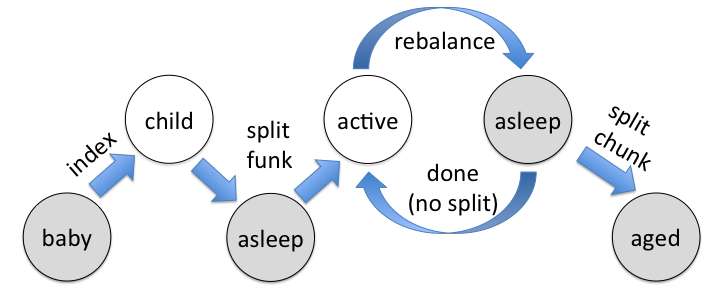
\includegraphics[width=\columnwidth]{state-diagram.png}
}
\caption{Chunk lifecycle; immutable states are grey and mutable ones are white.
Chunk splits  create new chunks in immutable \emph{baby} status, which changes to the mutable \emph{child} state once they 
are indexed. When the appropriate funks are created, the chunks become \emph{active}. All rebalance operations go through an 
\emph{asleep} state when the chunk is immutable.}
\label{fig:status}
\end{figure}

In the third case, the chunk is asleep when we create two new chunks to replace it. 
If the chunk has a munk, we split the munk (by creating two new munks) and update the appropriate pointers in the new chunks.  
Since creating new funks again involves I/O, we do not wish to keep the new chunks immutable for the duration of this process,
and allow funk creation to proceed in the background while the two new chunks still point to the same old funk. 

After we replace the old chunk in the list with the two new ones, 
the old chunk is still accessible via the chunk index (even though it is no longer in the list). 
The new chunks are therefore created in \emph{baby} status, indicating that they are still immutable. 
Once the new chunks are indexed, the old chunk is \emph{aged}, and the new chunks can become mutable.
At this point, we change their status to \emph{child}, indicating that they are no longer immutable, but share a funk with another chunk,
and so should not be rebalanced. Once the funk split completes, we put the chunks to sleep in order
to complete the funk switch and then change their  status  to active. 
The chunk's life-cycle is depicted in Figure~\ref{fig:status}.

\subsection{Disk flushes and recovery}
\label{ssec:flush-recovery}

Like most popular KV-stores, \sys\ supports two modes of operation -- \emph{synchronous} and \emph{asynchronous}. 
With the former,  updates are persisted to disk before returning to the user, and so a user is ensured when its operation
completes that the written data will survive failures. The drawback of this approach is that it is slow -- \inred{10x slower 
than the asynchronous mode in  existing KV-stores like RocksDB}. 
The asynchronous mode expedites updates by optimistically performing them in
RAM only and periodically \emph{flushing} them to disk. This reduces write latency and increases throughput, but 
may lead to loss of data that was written shortly before the crash. Since the tradeoffs between the two approaches are 
well known and the choice is typically left to the user, we support both modes in \sys.

In the synchronous mode, every put operation performs a flush after writing the data in the appropriate funk's \code{wbuf}, and then returns. 
This ensures that the funks always reflect all completed updates. In this case, recovery is straightforward: we simply construct
the chunks linked list from the funks on disk, and then the database can serve new requests, populating munks on-demand.  

In the asynchronous mode, we allow some suffix of the  data written before a crash to be lost, but always 
ensure that the data store \emph{consistently} reflects a \emph{prefix} of the  values written.
For example, if put(k1, v1) completes before put(k2, v2) and then the system crashes, then following the recovery, 
if k2 appears in the data store, then k1 must appear as well; conversely, if the update of k1 is lost, k2 must be also excluded.
Such recovery to a \emph{consistent snapshot} of the data store is important for applications where later updates may depend on earlier ones. 

\Idit{Add description of the background thread that takes a consistent snapshot, the incarnation numbers table, and the validation in gets} 

\remove{
\subsection{\sys\ operations}
\label{ssec:ops}

\inred{Consider if we want full pseudocode}
}








